\documentclass[12pt]{article}
\usepackage[margin=1in]{geometry}
\usepackage{booktabs}
\usepackage{graphicx}
\usepackage{setspace}
\usepackage{caption}
\usepackage{float}
\usepackage{microtype}
\usepackage{longtable}
\usepackage{array}
\usepackage[T1]{fontenc}
\usepackage{lmodern}
\usepackage{pdflscape}
\usepackage{needspace}
\usepackage[numbers,super,comma]{natbib}
\usepackage[hidelinks]{hyperref}
\captionsetup{font=footnotesize, labelfont=bf}
\setlength{\parskip}{6pt plus 2pt minus 1pt}
\doublespacing

\begin{document}
\raggedright

%% ── COVER PAGE ─────────────────────────────────────────────
\thispagestyle{empty}

\noindent\textbf{RESEARCH LETTER}

\vspace{24pt}

\noindent\textbf{Racism in Schools and Health Among US Adolescents in the United States, 2023}

\vspace{24pt}

\noindent Theodore L. Caputi\\
Massachusetts Institute of Technology, Department of Economics, Cambridge, MA

\vspace{24pt}

\noindent\textbf{Corresponding Author:} Theodore L. Caputi, MIT Department of Economics,
50 Memorial Dr, Cambridge, MA 02142 (tcaputi@gmail.com, https://www.tlcaputi.com).

\vspace{12pt}

\noindent\textbf{Conflict of Interest Disclosures:} TLC declares an equity
interest in Data Science Solutions, a public health consulting firm not
involved with this paper.

\vspace{12pt}

\noindent\textbf{Word Count:} 722

\clearpage

%% ── BODY ───────────────────────────────────────────────────
\noindent\textbf{Introduction}

Racism is one of the best documented and most powerful social determinants of
health.\cite{williams2013racism,paradies2015racism} However, there has been relatively little research studying the role
that racism plays in the health of children.\cite{priest2013racism} In this study, we examine the
relationship between experiences with racism at school and important health behaviors
among a nationally representative sample of US high school students.

\vspace{6pt}

\noindent\textbf{Methods}

This study uses data from the Centers for Disease Control and Prevention's 2023
Youth Risk Behavior Surveillance System (YRBS; $N = 20,103$; overall response rate
35.4\%), a biannual survey administered in US high schools on behavioral health
topics.\cite{cdc2023yrbs} The survey uses a three-stage cluster design to capture a representative
sample of high school students. The survey includes measures of mental health, substance
use, and violence victimization, among other important health behaviors (eTable 1 in the
Supplement). In 2023, the national YRBS introduced a measure of children's experience
with racism at school. Children were asked ``How often have you felt that you were treated
badly or unfairly in school because of your race or ethnicity?'' with possible responses
``Never,'' ``Rarely,'' ``Sometimes,'' ``Most of the time,'' and ``Always.''

First, the unadjusted prevalence of several risky behaviors is reported by level of
experience with racism. Then, the relative risk of each of these
behaviors was estimated via survey-weighted logistic regression, accounting for sex, age,
race/ethnicity, English language proficiency, and grades, relative to those who
experienced no racism.
These analyses were conducted collectively and by student race/ethnicity. Estimates are
presented as risk ratios, which are computed using random draws from the regression's
variance-covariance matrix and holding confounders at their means.\cite{king2000making}
All analyses account for the YRBS complex survey design to produce nationally
representative estimates and correct standard errors.

This study is exempt from institutional review as it only uses secondary analysis of
publicly available data.

\vspace{6pt}

\noindent\textbf{Results}

Of the 18,286 YRBS participants with non-missing data,
31.5\% (95\% CI, 29.0\%--34.1\%)
reported experiencing some racism at school, including
56.9\% of Asian,
45.9\% of Black,
42.5\% of Multiracial,
36.4\% of Hispanic, and
17.3\% of White children (\autoref{tab:main}).
5.7\% of non-White children reported experiencing racism at school most of the
time or always.

Most negative health behaviors exhibit a dose-response relationship with children's
experience with racism. For example, suicidal
ideation has a prevalence of 16.8\% among children who report never
experiencing racism, 25.6\% among children who report experiencing racism rarely
or sometimes, and 42.7\% among children who report experiencing racism most of
the time or always.

These patterns persist after accounting for potential confounders (\autoref{fig:rr}). After controlling for
sex, age, race/ethnicity, English language proficiency, and grades, those who experience
racism rarely or sometimes (RR 2.26, 95\% CI
1.87--2.67) and those who experience racism most of the time
or always (RR 4.42, 95\% CI
3.64--5.33) are significantly more likely to be bullied at
school compared with those who never experience racism. The response is strongest for
Asian children (rarely or sometimes RR 3.81, 95\% CI 1.23--11.61; most of the time or always RR 26.75, 95\% CI 8.15--73.83) and Black children (rarely or sometimes RR 2.87, 95\% CI 1.97--4.36; most of the time or always RR 6.61, 95\% CI 3.92--10.62) (eTable 2 in the Supplement).

\vspace{6pt}

\noindent\textbf{Discussion}

A significant proportion of US high school children report experiencing racism in schools,
and these experiences correlate significantly and in a dose-response relationship with
several negative health outcomes.

Racism is a well-recognized threat to public health.\cite{williams2013racism,paradies2015racism} These results extend that
finding to children in schools\cite{priest2013racism} and merit a well-coordinated response from public
health professionals. Recent studies find that a composite measure of racial mistreatment and school connection is strongly correlated with substance use and mental health behaviors among American adolescents. \cite{azagba2025school,azagba2026belonging} The present study complements these findings by examining a broader
set of health outcomes in a larger, nationally representative sample. Policy-makers, educators, and clinicians
may design interventions to reduce racism among young people and to screen children who
experience racism at school for negative health behaviors.\cite{trent2019impact}

This study has several limitations. This cross-sectional study cannot establish causation.
The YRBS is designed to be nationally representative, but its 35.4\% response rate could
limit generalizability. Though children respond privately and anonymously, self-report
can be biased. The survey uses multiple choice responses, which precludes more detailed
accounts of children's experience with racism. The survey did not capture student
experiences with racism outside of school.

Future research should seek a clearer understanding of how children experience racism
at school, the causal effects of racism on child health, and which policies and
interventions can reduce children's experience with racism.

%% ── REFERENCES ─────────────────────────────────────────────
\clearpage
\bibliographystyle{unsrtnat}
\bibliography{references}

%% ── TABLE (landscape) ──────────────────────────────────────
\begin{landscape}
\begin{table}[p]
\centering
\caption{Weighted Prevalence (\%) of Health Outcomes by Frequency of School-Based Racial Discrimination, 2023 YRBS}
\label{tab:main}
\footnotesize
\renewcommand{\arraystretch}{0.88}

\textbf{Panel A: Full Sample ($N = 18,286$)}
\vspace{4pt}

\begin{tabular}{l r ccccc}
\toprule
 & & \multicolumn{5}{c}{Weighted Prevalence, \% (95\% CI)} \\
\cmidrule(lr){3-7}
Outcome & $N$ & Never & Rarely & Sometimes & Most of the time & Always \\
 & & ($n = 12,530$) & ($n = 2,836$) & ($n = 2,024$) & ($n = 471$) & ($n = 425$) \\
\midrule
\textit{Mental Health} \\
\quad Persistent sadness or hopelessness & 18,094 & 33.8 (31.8--35.7) & 48.8 (45.4--52.2) & 58.1 (54.9--61.2) & 68.8 (62.5--75.0) & 62.2 (55.6--68.8) \\
\quad Seriously considered suicide & 18,025 & 16.8 (15.2--18.3) & 22.6 (20.1--25.2) & 30.0 (26.5--33.6) & 43.7 (36.2--51.1) & 41.7 (32.8--50.6) \\
\quad Made a suicide plan & 16,789 & 13.4 (11.7--15.1) & 19.8 (16.1--23.4) & 23.6 (19.4--27.8) & 39.3 (30.5--48.2) & 34.1 (25.7--42.4) \\
\quad Attempted suicide & 17,590 & 6.7 (5.8--7.7) & 11.0 (9.0--13.1) & 15.5 (13.3--17.6) & 26.1 (18.1--34.1) & 33.0 (24.1--41.9) \\
\addlinespace[4pt]
\textit{Violence} \\
\quad Bullied at school & 18,169 & 14.8 (13.0--16.6) & 20.2 (17.0--23.3) & 32.3 (27.4--37.1) & 47.5 (39.5--55.6) & 56.6 (48.9--64.3) \\
\quad Electronically bullied & 18,141 & 12.8 (11.2--14.5) & 18.0 (13.9--22.0) & 24.9 (20.7--29.1) & 39.7 (28.5--50.9) & 45.1 (36.1--54.2) \\
\quad Physical fight at school & 17,176 & 5.9 (5.1--6.7) & 9.1 (7.5--10.8) & 12.5 (10.4--14.6) & 17.2 (11.6--22.7) & 35.8 (29.0--42.5) \\
\quad Carried weapon at school & 17,813 & 3.1 (2.1--4.0) & 4.0 (2.8--5.3) & 5.8 (3.6--8.1) & 12.5 (7.4--17.5) & 18.8 (13.3--24.3) \\
\addlinespace[4pt]
\textit{Substance Use} \\
\quad Current cigarette use & 17,974 & 2.9 (2.2--3.7) & 3.5 (2.1--4.8) & 3.1 (1.7--4.5) & 7.4 (3.7--11.2) & 18.0 (11.3--24.7) \\
\quad Current e-cigarette use & 17,432 & 14.7 (13.2--16.1) & 18.4 (16.0--20.9) & 18.8 (15.6--22.0) & 28.5 (22.1--34.9) & 35.4 (27.7--43.2) \\
\quad Current alcohol use & 17,486 & 20.0 (18.1--22.0) & 25.8 (23.0--28.7) & 24.1 (20.5--27.6) & 29.9 (23.6--36.1) & 41.7 (32.4--51.0) \\
\quad Current marijuana use & 17,843 & 14.5 (13.1--16.0) & 19.5 (16.5--22.5) & 21.5 (17.6--25.5) & 29.9 (21.3--38.4) & 33.5 (24.9--42.2) \\
\bottomrule
\end{tabular}

\vspace{8pt}

\textbf{Panel B: Non-White Students ($N = 9,312$)}
\vspace{2pt}

\begin{tabular}{l r ccccc}
\toprule
 & & \multicolumn{5}{c}{Weighted Prevalence, \% (95\% CI)} \\
\cmidrule(lr){3-7}
Outcome & $N$ & Never & Rarely & Sometimes & Most of the time & Always \\
 & & ($n = 5,185$) & ($n = 1,926$) & ($n = 1,547$) & ($n = 349$) & ($n = 305$) \\
\midrule
\textit{Mental Health} \\
\quad Persistent sadness or hopelessness & 9,196 & 30.7 (28.5--33.0) & 48.8 (44.8--52.8) & 57.2 (53.4--61.0) & 67.3 (59.7--74.9) & 63.4 (56.8--69.9) \\
\quad Seriously considered suicide & 9,151 & 12.7 (11.4--14.1) & 21.3 (18.7--23.8) & 27.9 (24.1--31.8) & 43.1 (35.1--51.1) & 41.9 (29.9--53.9) \\
\quad Made a suicide plan & 8,953 & 11.5 (9.8--13.1) & 17.7 (15.0--20.4) & 22.5 (18.1--26.9) & 40.5 (33.4--47.5) & 30.2 (21.4--39.0) \\
\quad Attempted suicide & 8,904 & 6.3 (5.1--7.6) & 11.0 (8.8--13.3) & 16.3 (13.9--18.7) & 28.6 (20.3--37.0) & 34.0 (23.8--44.1) \\
\addlinespace[4pt]
\textit{Violence} \\
\quad Bullied at school & 9,248 & 8.7 (7.0--10.5) & 16.5 (13.0--20.0) & 27.7 (23.0--32.5) & 45.0 (36.4--53.6) & 55.3 (46.5--64.1) \\
\quad Electronically bullied & 9,225 & 8.2 (6.5--9.9) & 14.7 (11.3--18.1) & 20.5 (16.5--24.6) & 37.0 (27.5--46.5) & 41.5 (31.2--51.9) \\
\quad Physical fight at school & 8,627 & 6.7 (5.2--8.2) & 9.0 (6.9--11.2) & 12.2 (9.9--14.5) & 16.8 (10.4--23.2) & 35.7 (28.3--43.1) \\
\quad Carried weapon at school & 8,938 & 2.3 (1.6--3.0) & 3.3 (2.2--4.4) & 5.1 (3.1--7.2) & 10.0 (4.9--15.2) & 16.0 (9.6--22.5) \\
\addlinespace[4pt]
\textit{Substance Use} \\
\quad Current cigarette use & 9,119 & 1.4 (0.8--2.0) & 2.1 (0.9--3.2) & 1.7 (0.7--2.7) & 6.4 (2.4--10.5) & 17.0 (10.5--23.6) \\
\quad Current e-cigarette use & 8,798 & 11.8 (10.2--13.3) & 17.0 (14.5--19.6) & 17.5 (14.4--20.7) & 30.3 (23.1--37.5) & 39.0 (29.5--48.5) \\
\quad Current alcohol use & 8,857 & 14.9 (13.3--16.5) & 23.9 (20.8--27.1) & 21.1 (17.6--24.7) & 32.4 (25.0--39.7) & 40.7 (28.6--52.7) \\
\quad Current marijuana use & 9,034 & 12.9 (11.4--14.4) & 19.0 (15.7--22.2) & 20.8 (17.1--24.5) & 34.0 (23.5--44.5) & 37.5 (25.4--49.6) \\
\bottomrule
\end{tabular}

\vspace{4pt}
\begin{minipage}{\linewidth}
\scriptsize
\textit{Note.} CI = confidence interval. $N$ = unweighted analytic sample.
$n$ = unweighted students at each level of school-based racial discrimination.
Prevalences are weighted to the YRBS complex three-stage cluster design.
\end{minipage}

\end{table}
\end{landscape}

%% ── FIGURE (landscape) ─────────────────────────────────────
\begin{landscape}
\begin{figure}[H]
  \centering
  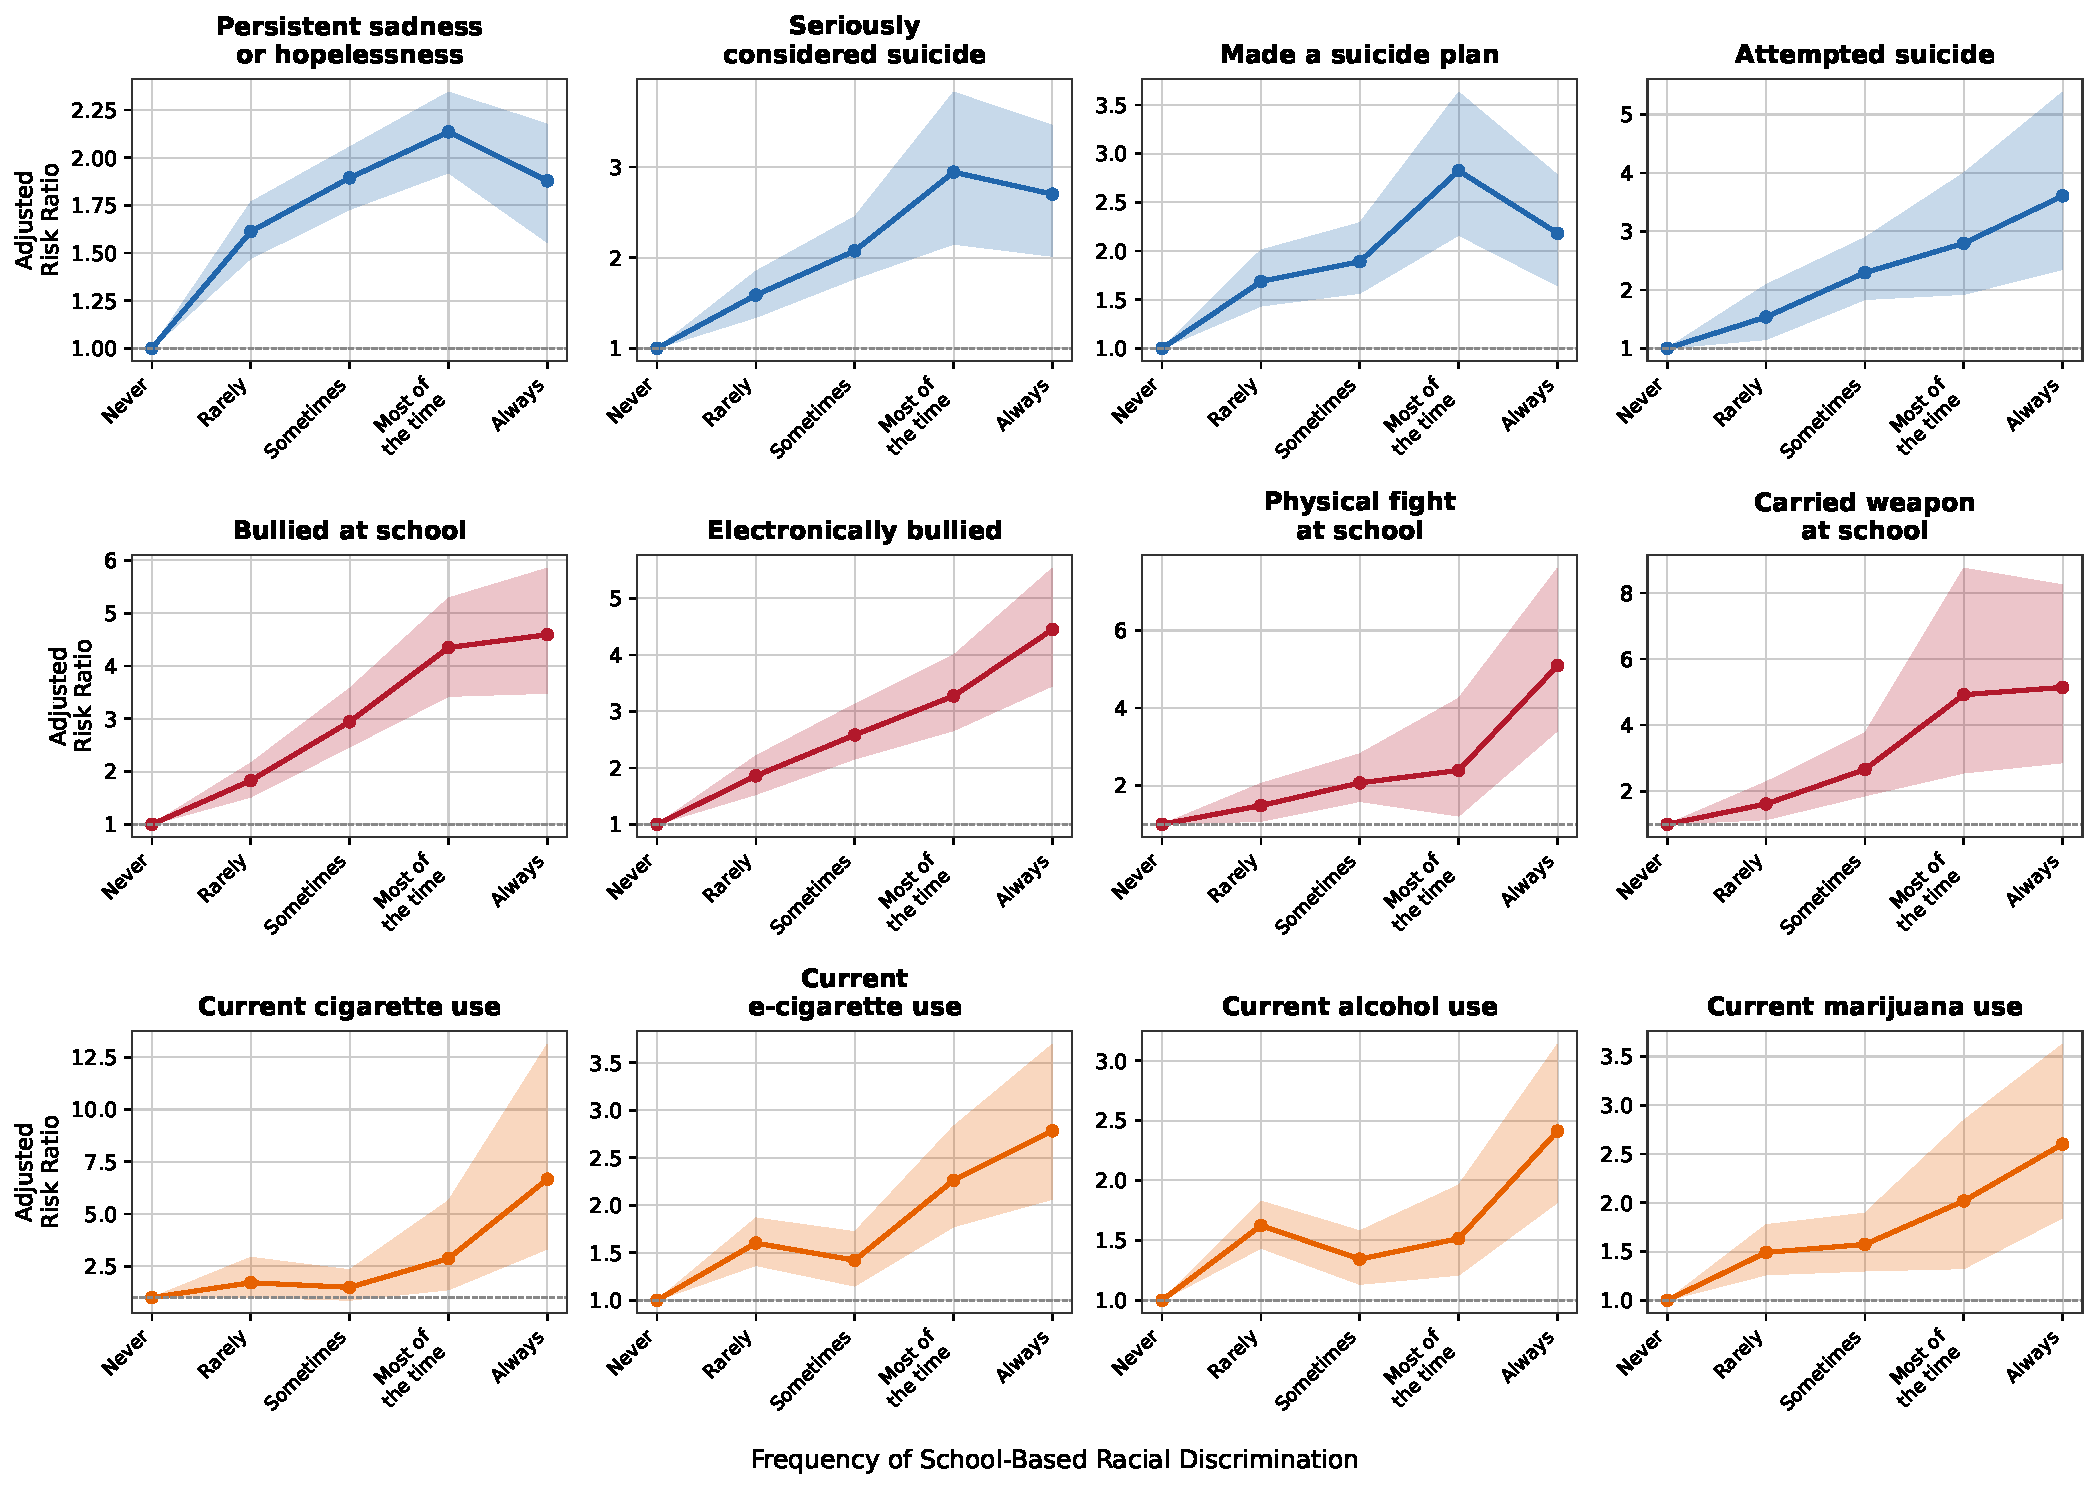
\includegraphics[width=\linewidth]{figures/figure1.pdf}
  \caption{Adjusted risk ratios for health outcomes by frequency of school-based
  racism among US high school students, 2023 YRBS ($N = 18,286$).
  Risk ratios from logistic regression computed via simulation from the
  variance-covariance matrix (King et al, 2000), adjusting for sex, age,
  race/ethnicity, English language proficiency, and grades.
  Shaded bands indicate 95\% confidence intervals. Reference category is Never.}
  \label{fig:rr}
\end{figure}
\end{landscape}

%% ── SUPPLEMENT ──────────────────────────────────────────────
\clearpage
\setcounter{page}{1}


\begin{landscape}
\singlespacing
\noindent\textbf{Supplement}\par
\vspace{6pt}
\noindent The 2023 National YRBS had an overall response rate of 35.4\% (school response rate 49.8\% $\times$ student response rate 71.0\%).\cite{cdc2023yrbs}\par
\vspace{8pt}
\noindent\textbf{eTable 1.} Survey Items and Analytic Coding, 2023 National Youth Risk Behavior Survey\par
\vspace{6pt}
\footnotesize
\renewcommand{\arraystretch}{1.1}
\begin{longtable}{>{\raggedright\arraybackslash}p{2.2in} >{\raggedright\arraybackslash}p{4.0in} >{\raggedright\arraybackslash}p{2.8in}}
\toprule
\textbf{Variable} & \textbf{Survey Question} & \textbf{Response Options / Coding} \\
\midrule
\endfirsthead
\toprule
\textbf{Variable} & \textbf{Survey Question} & \textbf{Response Options / Coding} \\
\midrule
\endhead
\bottomrule
\endfoot

\textit{Exposure} \\
\addlinespace[2pt]

School-based racism (Q23) &
``During your life, how often have you felt that you were treated badly or unfairly
in school because of your race or ethnicity?'' &
1 = Never; 2 = Rarely; 3 = Sometimes; 4 = Most of the time; 5 = Always.
Coded as categorical (5 levels; reference = Never). \\

\addlinespace[6pt]
\textit{Outcomes --- Mental Health} \\
\addlinespace[2pt]

Persistent sadness (QN26) &
``During the past 12 months, did you ever feel so sad or hopeless almost every day for
two weeks or more in a row that you stopped doing some usual activities?'' &
Yes / No. Coded as binary. \\
\addlinespace[3pt]

Suicidal ideation (QN27) &
``During the past 12 months, did you ever seriously consider attempting suicide?'' &
Yes / No. Coded as binary. \\
\addlinespace[3pt]

Suicide plan (QN28) &
``During the past 12 months, did you make a plan about how you would attempt suicide?'' &
Yes / No. Coded as binary. \\
\addlinespace[3pt]

Suicide attempt (QN29) &
``During the past 12 months, how many times did you actually attempt suicide?'' &
0 times / 1 time / 2--3 / 4--5 / 6+.
Coded as binary (1 if $\geq$1 time). \\

\addlinespace[6pt]
\textit{Outcomes --- Violence} \\
\addlinespace[2pt]

Bullied at school (QN24) &
``During the past 12 months, have you ever been bullied on school property?'' &
Yes / No. Coded as binary. \\
\addlinespace[3pt]

Electronically bullied (QN25) &
``During the past 12 months, have you ever been electronically bullied (counting being
bullied through texting, Instagram, Facebook, or other social media)?'' &
Yes / No. Coded as binary. \\
\addlinespace[3pt]

Physical fight at school (QN17) &
``During the past 12 months, how many times were you in a physical fight on school
property?'' &
0 / 1 / 2--3 / 4--5 / 6--7 / 8--9 / 10--11 / 12+ times.
Coded as binary (1 if $\geq$1 time). \\
\addlinespace[3pt]

Carried weapon at school (QN12) &
``During the past 30 days, on how many days did you carry a weapon such as a gun,
knife, or club on school property?'' &
0 / 1 / 2--3 / 4--5 / 6+ days.
Coded as binary (1 if $\geq$1 day). \\

\addlinespace[6pt]
\textit{Outcomes --- Substance Use} \\
\addlinespace[2pt]

Current cigarette use (QN33) &
``During the past 30 days, on how many days did you smoke cigarettes?'' &
0 / 1--2 / 3--5 / 6--9 / 10--19 / 20--29 / All 30 days.
Coded as binary (1 if $\geq$1 day). \\
\addlinespace[3pt]

Current e-cigarette use (QN36) &
``During the past 30 days, on how many days did you use an electronic vapor product?'' &
0 / 1--2 / 3--5 / 6--9 / 10--19 / 20--29 / All 30 days.
Coded as binary (1 if $\geq$1 day). \\
\addlinespace[3pt]

Current alcohol use (QN42) &
``During the past 30 days, on how many days did you have at least one drink of
alcohol?'' &
0 / 1--2 / 3--5 / 6--9 / 10--19 / 20--29 / All 30 days.
Coded as binary (1 if $\geq$1 day). \\
\addlinespace[3pt]

Current marijuana use (QN48) &
``During the past 30 days, how many times did you use marijuana?'' &
0 / 1--2 / 3--9 / 10--19 / 20--39 / 40+ times.
Coded as binary (1 if $\geq$1 time). \\

\addlinespace[6pt]
\textit{Covariates} \\
\addlinespace[2pt]

Sex (Q2) &
``What is your sex?'' &
Female / Male. Coded as binary (1 = Female). \\
\addlinespace[3pt]

Age (Q1) &
``How old are you?'' &
12 years or younger / 13 / 14 / 15 / 16 / 17 / 18 or older.
Coded as categorical (5 levels: $\leq$14, 15, 16, 17, 18+; ages $\leq$14 collapsed
because of sparse counts at 12 and 13). \\
\addlinespace[3pt]

Race/ethnicity (raceeth) &
Derived from Q4 (``Are you Hispanic or Latino?'') and Q5 (``What is your race?''). &
8 categories: AI/AN, Asian, Black, NH/PI, White, Hispanic, Multiple-Hispanic,
Multiple-Non-Hispanic.
Coded as categorical (8 levels). \\
\addlinespace[3pt]

Grades (QN87) &
``During the past 12 months, how would you describe your grades in school?'' &
Mostly A's / B's / C's / D's / F's / None / Not sure.
Coded as binary (1 if A's or B's). \\
\addlinespace[3pt]

English proficiency (QN107) &
``How well do you speak English?'' &
Very well / Well / Not well / Not at all.
Coded as binary (1 if Very well or Well). \\

\end{longtable}
\doublespacing
\normalsize
\end{landscape}


\begin{landscape}
\footnotesize
\noindent\textbf{eTable 2.} Adjusted Risk Ratios for Health Outcomes by Frequency of School-Based Racial Discrimination, Stratified by Race/Ethnicity, 2023 YRBS\par
\vspace{6pt}
\nobreak\noindent\textbf{All Students ($N = 18,286$)}
\nopagebreak\par\nopagebreak\vspace{1pt}\nopagebreak
\nobreak\noindent\begin{tabular}{l r ccccc}
\toprule
 & & \multicolumn{5}{c}{Adjusted Risk Ratio (95\% CI)} \\
\cmidrule(lr){3-7}
Outcome & $N$ & Never & Rarely & Sometimes & Most of the time & Always \\
\midrule
\textit{Mental Health} \\
\quad Persistent sadness or hopelessness & 10,299 & 1 [Ref] & 1.61 (1.47--1.77) & 1.89 (1.73--2.06) & 2.14 (1.92--2.34) & 1.88 (1.56--2.18) \\
\quad Seriously considered suicide & 10,263 & 1 [Ref] & 1.59 (1.34--1.85) & 2.08 (1.77--2.45) & 2.94 (2.15--3.83) & 2.70 (2.02--3.46) \\
\quad Made a suicide plan & 10,270 & 1 [Ref] & 1.69 (1.43--2.01) & 1.89 (1.57--2.29) & 2.82 (2.16--3.63) & 2.18 (1.64--2.78) \\
\quad Attempted suicide & 10,284 & 1 [Ref] & 1.54 (1.15--2.09) & 2.29 (1.83--2.89) & 2.80 (1.92--4.00) & 3.61 (2.35--5.38) \\
\addlinespace[4pt]
\textit{Violence} \\
\quad Bullied at school & 10,318 & 1 [Ref] & 1.83 (1.51--2.16) & 2.94 (2.47--3.58) & 4.35 (3.42--5.29) & 4.59 (3.48--5.85) \\
\quad Electronically bullied & 10,312 & 1 [Ref] & 1.86 (1.53--2.21) & 2.58 (2.16--3.13) & 3.27 (2.66--4.00) & 4.45 (3.45--5.54) \\
\quad Physical fight at school & 10,294 & 1 [Ref] & 1.48 (1.08--2.05) & 2.07 (1.59--2.82) & 2.39 (1.21--4.25) & 5.09 (3.41--7.61) \\
\quad Carried weapon at school & 10,334 & 1 [Ref] & 1.61 (1.14--2.28) & 2.66 (1.86--3.77) & 4.92 (2.55--8.75) & 5.14 (2.86--8.24) \\
\addlinespace[4pt]
\textit{Substance Use} \\
\quad Current cigarette use & 10,315 & 1 [Ref] & 1.71 (1.01--2.92) & 1.49 (0.87--2.33) & 2.87 (1.37--5.64) & 6.66 (3.33--13.13) \\
\quad Current e-cigarette use & 9,949 & 1 [Ref] & 1.60 (1.37--1.87) & 1.42 (1.15--1.72) & 2.26 (1.77--2.83) & 2.78 (2.06--3.70) \\
\quad Current alcohol use & 10,195 & 1 [Ref] & 1.62 (1.44--1.83) & 1.34 (1.13--1.58) & 1.52 (1.21--1.96) & 2.41 (1.82--3.14) \\
\quad Current marijuana use & 10,270 & 1 [Ref] & 1.49 (1.26--1.78) & 1.57 (1.30--1.89) & 2.02 (1.32--2.85) & 2.60 (1.85--3.63) \\
\bottomrule
\end{tabular}\par\vspace{8pt}

\nobreak\noindent\textbf{Non-White Students ($N = 9,312$)}
\nopagebreak\par\nopagebreak\vspace{1pt}\nopagebreak
\nobreak\noindent\begin{tabular}{l r ccccc}
\toprule
 & & \multicolumn{5}{c}{Adjusted Risk Ratio (95\% CI)} \\
\cmidrule(lr){3-7}
Outcome & $N$ & Never & Rarely & Sometimes & Most of the time & Always \\
\midrule
\textit{Mental Health} \\
\quad Persistent sadness or hopelessness & 5,797 & 1 [Ref] & 1.75 (1.57--1.95) & 1.96 (1.75--2.17) & 2.19 (1.88--2.52) & 2.03 (1.68--2.39) \\
\quad Seriously considered suicide & 5,775 & 1 [Ref] & 1.81 (1.50--2.19) & 2.28 (1.83--2.84) & 3.45 (2.35--4.86) & 3.29 (2.34--4.34) \\
\quad Made a suicide plan & 5,781 & 1 [Ref] & 1.80 (1.52--2.18) & 1.98 (1.58--2.46) & 3.49 (2.48--4.71) & 2.10 (1.54--2.80) \\
\quad Attempted suicide & 5,795 & 1 [Ref] & 1.69 (1.21--2.32) & 2.74 (2.05--3.60) & 3.45 (2.11--5.60) & 4.70 (3.27--6.79) \\
\addlinespace[4pt]
\textit{Violence} \\
\quad Bullied at school & 5,817 & 1 [Ref] & 2.33 (1.77--3.05) & 3.33 (2.50--4.32) & 5.85 (4.36--7.68) & 6.33 (4.74--8.69) \\
\quad Electronically bullied & 5,813 & 1 [Ref] & 2.19 (1.72--2.78) & 2.73 (2.12--3.50) & 3.93 (2.85--5.28) & 5.60 (3.76--7.90) \\
\quad Physical fight at school & 5,795 & 1 [Ref] & 1.56 (0.99--2.38) & 2.00 (1.37--2.79) & 1.98 (0.93--3.84) & 4.64 (3.24--6.98) \\
\quad Carried weapon at school & 5,823 & 1 [Ref] & 1.67 (0.87--3.20) & 3.28 (1.95--5.63) & 6.07 (3.11--11.50) & 7.12 (3.78--12.67) \\
\addlinespace[4pt]
\textit{Substance Use} \\
\quad Current cigarette use & 5,819 & 1 [Ref] & 1.85 (0.82--4.68) & 1.65 (0.73--3.72) & 3.30 (1.26--9.03) & 10.28 (5.03--19.92) \\
\quad Current e-cigarette use & 5,572 & 1 [Ref] & 1.74 (1.39--2.17) & 1.45 (1.10--1.87) & 2.47 (1.77--3.40) & 3.40 (2.47--4.56) \\
\quad Current alcohol use & 5,734 & 1 [Ref] & 1.81 (1.53--2.09) & 1.36 (1.09--1.68) & 1.73 (1.26--2.35) & 3.05 (2.05--4.19) \\
\quad Current marijuana use & 5,784 & 1 [Ref] & 1.56 (1.25--1.93) & 1.65 (1.32--2.12) & 2.31 (1.44--3.49) & 3.30 (2.08--4.64) \\
\bottomrule
\end{tabular}\par\vspace{8pt}

\nobreak\noindent\textbf{White Students ($N = 8,733$)}
\nopagebreak\par\nopagebreak\vspace{1pt}\nopagebreak
\nobreak\noindent\begin{tabular}{l r ccccc}
\toprule
 & & \multicolumn{5}{c}{Adjusted Risk Ratio (95\% CI)} \\
\cmidrule(lr){3-7}
Outcome & $N$ & Never & Rarely & Sometimes & Most of the time & Always \\
\midrule
\textit{Mental Health} \\
\quad Persistent sadness or hopelessness & 4,502 & 1 [Ref] & 1.39 (1.21--1.59) & 1.85 (1.51--2.16) & 2.11 (1.55--2.55) & 1.55 (0.78--2.20) \\
\quad Seriously considered suicide & 4,488 & 1 [Ref] & 1.31 (1.00--1.72) & 1.92 (1.59--2.29) & 2.37 (1.43--3.34) & 1.74 (1.10--2.61) \\
\quad Made a suicide plan & 4,489 & 1 [Ref] & 1.54 (1.08--2.15) & 1.75 (1.29--2.36) & 1.43 (0.67--2.64) & 2.43 (1.30--4.14) \\
\quad Attempted suicide & 4,489 & 1 [Ref] & 1.52 (0.93--2.52) & 1.53 (0.87--2.75) & 1.59 (0.87--2.87) & 1.22 (0.34--4.16) \\
\addlinespace[4pt]
\textit{Violence} \\
\quad Bullied at school & 4,501 & 1 [Ref] & 1.35 (1.05--1.74) & 2.72 (2.21--3.31) & 3.01 (1.87--3.99) & 2.72 (1.11--4.27) \\
\quad Electronically bullied & 4,499 & 1 [Ref] & 1.49 (1.11--2.00) & 2.56 (1.88--3.37) & 2.75 (1.76--3.77) & 2.98 (1.60--4.51) \\
\quad Physical fight at school & 4,499 & 1 [Ref] & 1.22 (0.74--2.08) & 2.40 (1.45--3.94) & 3.74 (1.27--9.46) & 6.66 (2.79--12.55) \\
\quad Carried weapon at school & 4,511 & 1 [Ref] & 1.65 (1.13--2.34) & 1.94 (1.23--3.07) & 4.77 (2.15--9.50) & 3.09 (1.30--6.84) \\
\addlinespace[4pt]
\textit{Substance Use} \\
\quad Current cigarette use & 4,496 & 1 [Ref] & 1.64 (0.99--2.84) & 1.40 (0.68--2.83) & 2.16 (0.63--6.81) & 2.85 (0.65--10.11) \\
\quad Current e-cigarette use & 4,377 & 1 [Ref] & 1.40 (1.06--1.80) & 1.46 (1.03--2.06) & 1.75 (1.07--2.83) & 1.64 (0.59--3.63) \\
\quad Current alcohol use & 4,461 & 1 [Ref] & 1.36 (1.06--1.71) & 1.34 (1.06--1.69) & 1.08 (0.60--1.68) & 1.60 (0.83--2.67) \\
\quad Current marijuana use & 4,486 & 1 [Ref] & 1.38 (1.03--1.81) & 1.48 (1.05--2.02) & 1.39 (0.86--2.17) & 1.29 (0.35--3.40) \\
\bottomrule
\end{tabular}\par\vspace{8pt}

\nobreak\noindent\textbf{Black Students ($N = 1,732$)}
\nopagebreak\par\nopagebreak\vspace{1pt}\nopagebreak
\nobreak\noindent\begin{tabular}{l r ccccc}
\toprule
 & & \multicolumn{5}{c}{Adjusted Risk Ratio (95\% CI)} \\
\cmidrule(lr){3-7}
Outcome & $N$ & Never & Rarely & Sometimes & Most of the time & Always \\
\midrule
\textit{Mental Health} \\
\quad Persistent sadness or hopelessness & 1,220 & 1 [Ref] & 1.62 (1.24--2.08) & 1.87 (1.48--2.35) & 2.43 (1.74--2.99) & 1.72 (1.10--2.47) \\
\quad Seriously considered suicide & 1,215 & 1 [Ref] & 1.63 (1.11--2.39) & 2.07 (1.35--3.12) & 3.12 (1.25--6.06) & 1.62 (0.70--3.19) \\
\quad Made a suicide plan & 1,221 & 1 [Ref] & 1.79 (1.33--2.39) & 1.75 (1.13--2.76) & 2.60 (0.80--6.45) & 2.45 (0.90--5.19) \\
\quad Attempted suicide & 1,220 & 1 [Ref] & 2.90 (1.70--5.04) & 3.02 (1.79--5.43) & 4.52 (1.28--12.28) & 2.80 (0.89--7.76) \\
\addlinespace[4pt]
\textit{Violence} \\
\quad Bullied at school & 1,221 & 1 [Ref] & 2.71 (1.61--4.30) & 3.10 (2.00--4.89) & 8.08 (4.17--13.33) & 5.83 (3.03--10.02) \\
\quad Electronically bullied & 1,219 & 1 [Ref] & 2.86 (1.87--4.42) & 1.91 (1.06--3.47) & 6.51 (2.51--13.21) & 3.90 (1.64--8.51) \\
\quad Physical fight at school & 1,212 & 1 [Ref] & 2.01 (1.13--3.50) & 1.08 (0.63--1.77) & 2.81 (0.76--7.01) & 4.20 (1.90--7.65) \\
\quad Carried weapon at school & 1,222 & 1 [Ref] & 0.57 (0.17--1.73) & 1.13 (0.42--3.06) & 12.40 (2.73--37.51) & 4.72 (1.59--12.35) \\
\addlinespace[4pt]
\textit{Substance Use} \\
\quad Current cigarette use & 1,225 & 1 [Ref] & 1.67 (0.21--14.15) & 0.87 (0.14--5.06) & 1.41 (0.08--23.15) & 6.68 (1.99--19.39) \\
\quad Current e-cigarette use & 1,163 & 1 [Ref] & 1.67 (1.01--2.73) & 1.71 (1.15--2.47) & 2.51 (0.65--6.72) & 4.15 (2.75--5.95) \\
\quad Current alcohol use & 1,204 & 1 [Ref] & 2.13 (1.30--3.37) & 1.40 (0.90--2.01) & 2.16 (0.85--4.60) & 3.35 (1.49--5.91) \\
\quad Current marijuana use & 1,221 & 1 [Ref] & 1.81 (1.23--2.60) & 1.90 (1.39--2.67) & 2.95 (1.22--5.40) & 2.86 (1.63--4.63) \\
\bottomrule
\end{tabular}\par\vspace{8pt}

\nobreak\noindent\textbf{Hispanic Students ($N = 1,179$)}
\nopagebreak\par\nopagebreak\vspace{1pt}\nopagebreak
\nobreak\noindent\begin{tabular}{l r ccccc}
\toprule
 & & \multicolumn{5}{c}{Adjusted Risk Ratio (95\% CI)} \\
\cmidrule(lr){3-7}
Outcome & $N$ & Never & Rarely & Sometimes & Most of the time & Always \\
\midrule
\textit{Mental Health} \\
\quad Persistent sadness or hopelessness & 569 & 1 [Ref] & 1.96 (1.39--2.89) & 2.29 (1.72--3.16) & 3.43 (2.63--4.58) & 1.07 (0.26--2.53) \\
\quad Seriously considered suicide & 561 & 1 [Ref] & 2.32 (1.18--4.55) & 3.05 (2.04--4.49) & 8.68 (1.73--16.37) & 2.60 (0.31--9.83) \\
\quad Made a suicide plan & 568 & 1 [Ref] & 3.10 (1.96--4.88) & 4.61 (2.63--7.76) & 9.49 (2.53--16.59) & 0.00 (0.00--0.00) \\
\quad Attempted suicide & 563 & 1 [Ref] & 1.31 (0.61--2.78) & 3.13 (1.40--7.38) & 5.46 (1.63--12.94) & 2.41 (0.16--14.26) \\
\addlinespace[4pt]
\textit{Violence} \\
\quad Bullied at school & 571 & 1 [Ref] & 1.35 (0.73--2.52) & 2.02 (1.00--4.09) & 3.72 (0.66--10.19) & 3.54 (0.76--11.54) \\
\quad Electronically bullied & 569 & 1 [Ref] & 2.28 (0.84--5.68) & 2.53 (0.98--5.89) & 8.15 (1.43--21.88) & 1.94 (0.17--11.52) \\
\quad Physical fight at school & 573 & 1 [Ref] & 1.00 (0.34--3.17) & 3.05 (1.23--7.19) & 0.89 (0.12--4.78) & 0.00 (0.00--0.00) \\
\quad Carried weapon at school & 569 & 1 [Ref] & 10.85 (3.07--35.82) & 11.26 (2.14--60.62) & 0.94 (0.09--10.12) & 0.00 (0.00--0.00) \\
\addlinespace[4pt]
\textit{Substance Use} \\
\quad Current cigarette use & 572 & 1 [Ref] & 0.00 (0.00--0.00) & 0.04 (0.00--0.46) & --- & 0.00 (0.00--0.00) \\
\quad Current e-cigarette use & 552 & 1 [Ref] & 2.20 (1.28--3.70) & 0.89 (0.45--1.66) & 2.93 (0.57--8.85) & 1.53 (0.17--6.94) \\
\quad Current alcohol use & 566 & 1 [Ref] & 2.54 (1.55--4.26) & 2.17 (1.26--3.61) & 1.81 (0.52--4.64) & 2.58 (0.38--8.79) \\
\quad Current marijuana use & 568 & 1 [Ref] & 2.12 (1.07--3.96) & 0.35 (0.11--1.25) & 2.33 (0.39--9.54) & 3.62 (0.69--12.75) \\
\bottomrule
\end{tabular}\par\vspace{8pt}

\nobreak\noindent\textbf{Asian Students ($N = 927$)}
\nopagebreak\par\nopagebreak\vspace{1pt}\nopagebreak
\nobreak\noindent\begin{tabular}{l r ccccc}
\toprule
 & & \multicolumn{5}{c}{Adjusted Risk Ratio (95\% CI)} \\
\cmidrule(lr){3-7}
Outcome & $N$ & Never & Rarely & Sometimes & Most of the time & Always \\
\midrule
\textit{Mental Health} \\
\quad Persistent sadness or hopelessness & 396 & 1 [Ref] & 2.44 (1.66--3.53) & 3.35 (2.28--4.79) & 4.25 (2.34--6.67) & 5.40 (2.88--7.82) \\
\quad Seriously considered suicide & 393 & 1 [Ref] & 4.08 (1.77--11.04) & 6.97 (2.08--23.84) & 12.80 (3.05--45.10) & 13.39 (3.26--48.98) \\
\quad Made a suicide plan & 392 & 1 [Ref] & 3.23 (1.12--11.81) & 1.47 (0.52--4.71) & 10.71 (3.40--31.84) & 2.57 (0.31--15.24) \\
\quad Attempted suicide & 397 & 1 [Ref] & 1.21 (0.31--4.58) & 3.15 (1.25--7.56) & 16.65 (5.26--49.32) & 6.65 (1.04--29.62) \\
\addlinespace[4pt]
\textit{Violence} \\
\quad Bullied at school & 394 & 1 [Ref] & 1.79 (0.43--6.83) & 8.55 (2.42--28.47) & 20.19 (4.99--64.42) & --- \\
\quad Electronically bullied & 396 & 1 [Ref] & 2.23 (0.71--6.43) & 5.09 (1.49--15.78) & 1.35 (0.27--6.65) & 12.34 (2.74--36.51) \\
\quad Physical fight at school & 398 & 1 [Ref] & 1.07 (0.23--4.74) & 4.36 (0.48--45.21) & --- & 0.62 (0.02--13.01) \\
\quad Carried weapon at school & 398 & 1 [Ref] & 0.78 (0.04--13.45) & 15.89 (2.01--99.18) & --- & 0.00 (0.00--0.00) \\
\addlinespace[4pt]
\textit{Substance Use} \\
\quad Current cigarette use & 396 & 1 [Ref] & --- & --- & --- & --- \\
\quad Current e-cigarette use & 389 & 1 [Ref] & 2.69 (0.66--10.51) & 6.08 (0.66--48.74) & --- & 1.82 (0.13--20.66) \\
\quad Current alcohol use & 399 & 1 [Ref] & 0.94 (0.36--2.32) & 2.43 (1.28--4.43) & 2.65 (0.27--11.58) & 2.72 (0.31--10.48) \\
\quad Current marijuana use & 395 & 1 [Ref] & 0.76 (0.13--3.99) & 3.51 (0.78--17.58) & 2.70 (0.35--14.60) & 0.14 (0.01--1.93) \\
\bottomrule
\end{tabular}\par\vspace{8pt}

\nobreak\noindent\textbf{American Indian/Alaska Native Students ($N = 1,086$)}
\nopagebreak\par\nopagebreak\vspace{1pt}\nopagebreak
\nobreak\noindent\begin{tabular}{l r ccccc}
\toprule
 & & \multicolumn{5}{c}{Adjusted Risk Ratio (95\% CI)} \\
\cmidrule(lr){3-7}
Outcome & $N$ & Never & Rarely & Sometimes & Most of the time & Always \\
\midrule
\textit{Mental Health} \\
\quad Persistent sadness or hopelessness & 821 & 1 [Ref] & 1.64 (1.05--2.63) & 1.09 (0.46--1.91) & 1.81 (0.99--2.85) & 1.84 (1.11--2.95) \\
\quad Seriously considered suicide & 817 & 1 [Ref] & 2.16 (0.88--5.09) & 2.15 (0.61--6.84) & 6.31 (2.90--13.00) & 1.46 (0.17--7.12) \\
\quad Made a suicide plan & 815 & 1 [Ref] & 0.71 (0.22--2.16) & 2.86 (0.98--6.86) & 5.77 (2.57--11.22) & 1.57 (0.22--6.32) \\
\quad Attempted suicide & 820 & 1 [Ref] & 2.61 (0.87--7.40) & 3.42 (0.56--15.58) & 14.38 (5.60--34.57) & 13.51 (4.01--35.59) \\
\addlinespace[4pt]
\textit{Violence} \\
\quad Bullied at school & 822 & 1 [Ref] & 2.76 (0.88--7.82) & 7.49 (2.40--19.39) & 12.85 (4.57--31.68) & 23.67 (10.26--51.61) \\
\quad Electronically bullied & 822 & 1 [Ref] & 1.09 (0.28--3.38) & 2.57 (0.81--7.05) & 7.81 (4.06--13.57) & 8.30 (4.45--16.41) \\
\quad Physical fight at school & 816 & 1 [Ref] & 1.15 (0.44--2.73) & 0.31 (0.05--2.09) & 0.11 (0.01--2.37) & 1.86 (0.11--19.87) \\
\quad Carried weapon at school & 823 & 1 [Ref] & 1.76 (0.47--6.65) & 2.37 (0.57--8.62) & 2.28 (0.24--18.20) & 0.00 (0.00--0.00) \\
\addlinespace[4pt]
\textit{Substance Use} \\
\quad Current cigarette use & 821 & 1 [Ref] & 0.31 (0.06--1.74) & 1.18 (0.12--9.17) & 23.83 (5.57--68.14) & 2.42 (0.18--21.38) \\
\quad Current e-cigarette use & 780 & 1 [Ref] & 1.88 (0.70--4.34) & 1.07 (0.34--2.96) & 3.54 (1.78--6.26) & 0.80 (0.08--3.95) \\
\quad Current alcohol use & 796 & 1 [Ref] & 0.63 (0.17--1.97) & 2.63 (0.99--6.82) & 3.35 (0.75--8.31) & 3.32 (0.47--9.63) \\
\quad Current marijuana use & 818 & 1 [Ref] & 1.46 (0.50--3.43) & 1.64 (0.62--3.56) & 2.89 (1.29--5.32) & 1.50 (0.04--5.33) \\
\bottomrule
\end{tabular}\par\vspace{8pt}

\nobreak\noindent\textbf{Native Hawaiian/Pacific Islander Students ($N = 92$)}
\nopagebreak\par\nopagebreak\vspace{1pt}\nopagebreak
\nobreak\noindent\begin{tabular}{l r ccccc}
\toprule
 & & \multicolumn{5}{c}{Adjusted Risk Ratio (95\% CI)} \\
\cmidrule(lr){3-7}
Outcome & $N$ & Never & Rarely & Sometimes & Most of the time & Always \\
\midrule
\textit{Mental Health} \\
\quad Persistent sadness or hopelessness & 53 & 1 [Ref] & 0.75 (0.16--5.21) & 1.30 (0.09--8.35) & 0.00 (0.00--0.00) & 3.23 (1.34--13.71) \\
\quad Seriously considered suicide & 53 & 1 [Ref] & 0.74 (0.02--20.75) & --- & 0.00 (0.00--0.00) & --- \\
\quad Made a suicide plan & 53 & 1 [Ref] & --- & --- & 0.00 (0.00--0.00) & --- \\
\quad Attempted suicide & 53 & 1 [Ref] & --- & --- & 0.00 (0.00--0.00) & --- \\
\addlinespace[4pt]
\textit{Violence} \\
\quad Bullied at school & 53 & 1 [Ref] & --- & 0.00 (0.00--0.00) & --- & --- \\
\quad Electronically bullied & 53 & 1 [Ref] & --- & --- & --- & --- \\
\quad Physical fight at school & 53 & 1 [Ref] & --- & --- & --- & --- \\
\quad Carried weapon at school & 52 & 1 [Ref] & --- & --- & --- & --- \\
\addlinespace[4pt]
\textit{Substance Use} \\
\quad Current cigarette use & 53 & 1 [Ref] & --- & --- & --- & --- \\
\quad Current e-cigarette use & 51 & 1 [Ref] & 0.00 (0.00--0.00) & --- & 0.00 (0.00--0.00) & --- \\
\quad Current alcohol use & 51 & 1 [Ref] & --- & --- & 0.00 (0.00--0.00) & --- \\
\quad Current marijuana use & 53 & 1 [Ref] & 0.00 (0.00--0.00) & --- & 0.00 (0.00--0.00) & --- \\
\bottomrule
\end{tabular}\par\vspace{8pt}

\nobreak\noindent\textbf{Multiracial Students ($N = 4,296$)}
\nopagebreak\par\nopagebreak\vspace{1pt}\nopagebreak
\nobreak\noindent\begin{tabular}{l r ccccc}
\toprule
 & & \multicolumn{5}{c}{Adjusted Risk Ratio (95\% CI)} \\
\cmidrule(lr){3-7}
Outcome & $N$ & Never & Rarely & Sometimes & Most of the time & Always \\
\midrule
\textit{Mental Health} \\
\quad Persistent sadness or hopelessness & 2,738 & 1 [Ref] & 1.73 (1.51--1.97) & 1.87 (1.64--2.12) & 1.88 (1.52--2.27) & 2.11 (1.58--2.58) \\
\quad Seriously considered suicide & 2,736 & 1 [Ref] & 1.81 (1.34--2.39) & 2.21 (1.65--2.93) & 3.18 (2.21--4.41) & 3.90 (2.74--5.08) \\
\quad Made a suicide plan & 2,732 & 1 [Ref] & 1.52 (1.09--2.15) & 1.79 (1.34--2.33) & 2.88 (1.91--4.07) & 2.03 (1.19--3.31) \\
\quad Attempted suicide & 2,742 & 1 [Ref] & 1.48 (1.01--2.27) & 2.63 (1.78--3.81) & 2.68 (1.27--5.13) & 5.67 (3.57--8.31) \\
\addlinespace[4pt]
\textit{Violence} \\
\quad Bullied at school & 2,756 & 1 [Ref] & 2.58 (2.06--3.30) & 3.74 (2.93--4.72) & 5.33 (3.97--6.96) & 6.34 (4.67--8.25) \\
\quad Electronically bullied & 2,754 & 1 [Ref] & 2.01 (1.46--2.81) & 3.04 (2.24--4.14) & 3.26 (2.02--5.34) & 6.10 (3.60--9.18) \\
\quad Physical fight at school & 2,743 & 1 [Ref] & 1.41 (0.78--2.41) & 2.36 (1.31--4.01) & 1.02 (0.34--3.02) & 6.06 (3.42--11.07) \\
\quad Carried weapon at school & 2,759 & 1 [Ref] & 1.76 (0.85--3.54) & 3.40 (1.63--7.02) & 3.55 (1.51--7.28) & 7.85 (4.08--15.68) \\
\addlinespace[4pt]
\textit{Substance Use} \\
\quad Current cigarette use & 2,752 & 1 [Ref] & 2.18 (0.97--4.94) & 1.90 (0.70--4.77) & 2.65 (0.54--11.12) & 11.16 (5.05--23.91) \\
\quad Current e-cigarette use & 2,637 & 1 [Ref] & 1.68 (1.20--2.32) & 1.42 (1.02--1.90) & 2.15 (1.46--3.19) & 3.17 (1.98--4.61) \\
\quad Current alcohol use & 2,718 & 1 [Ref] & 1.69 (1.41--2.02) & 1.21 (0.83--1.74) & 1.63 (1.10--2.30) & 3.02 (1.86--4.34) \\
\quad Current marijuana use & 2,729 & 1 [Ref] & 1.52 (1.15--2.02) & 1.69 (1.31--2.23) & 2.21 (1.25--3.50) & 3.56 (2.13--5.15) \\
\bottomrule
\end{tabular}\par\vspace{8pt}

\normalsize
\end{landscape}

\begin{landscape}
\begin{figure}[H]
  \centering
  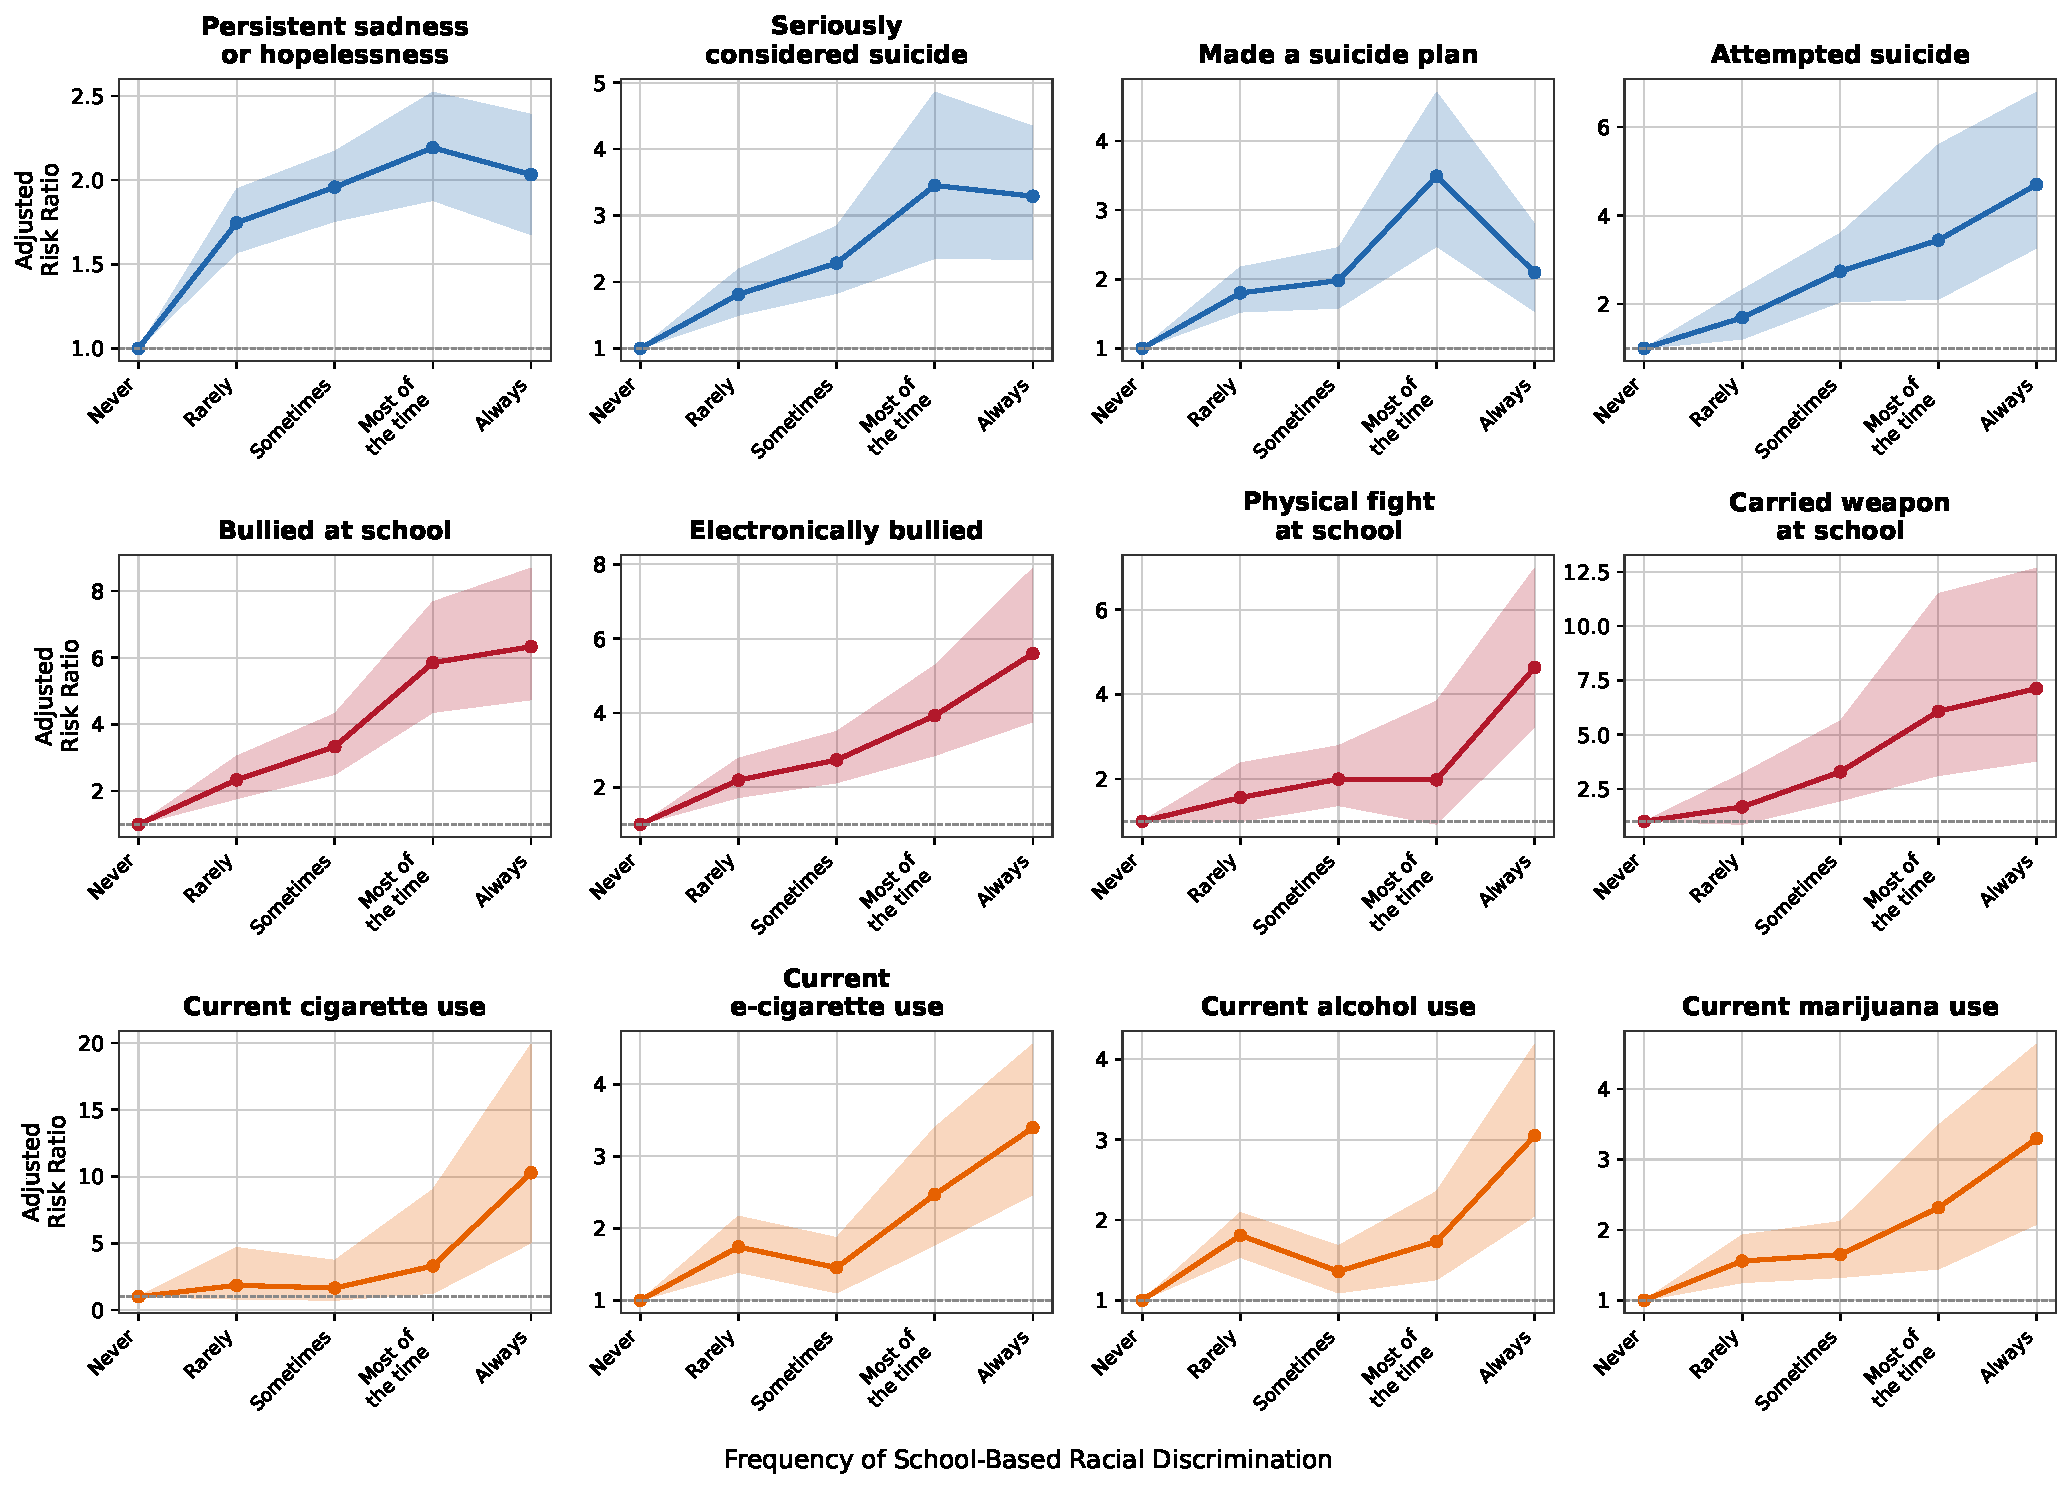
\includegraphics[width=\linewidth]{figures/efigure1.pdf}
  \caption*{\textbf{eFigure 1.} Adjusted risk ratios for health outcomes by frequency of school-based
  racism among non-White US high school students, 2023 YRBS ($N = 9,312$).
  Risk ratios from logistic regression computed via simulation from the
  variance-covariance matrix (King et al, 2000), adjusting for sex, age,
  race/ethnicity, English language proficiency, and grades.
  Shaded bands indicate 95\% confidence intervals. Reference category is Never.}
  \label{fig:efig1}
\end{figure}

\vspace{6pt}

\noindent\textbf{Data and Code Availability.} Data are publicly available from the Centers
for Disease Control and Prevention.\cite{cdc2023yrbs} Code to download the data and reproduce all analyses is
available at \url{https://github.com/tlcaputi/yrbs-racism}.
\end{landscape}

\end{document}
